



\usetikzlibrary{arrows, decorations.markings}
\usetikzlibrary{trees}

\tikzstyle{level 1}=[level distance=1cm, sibling distance=1.5cm]
\tikzstyle{level 2}=[level distance=1cm, sibling distance=1.1cm]

% Define styles for operators and leafs
\tikzstyle{operator} = [draw=none,circle, minimum width=1pt]
\tikzstyle{end} = [circle, minimum width=3pt,fill, inner sep=0pt]
% for double arrows a la chef
% adapt line thickness and line width, if needed

\begin{subfigure}[b]{0.49\textwidth}\centering
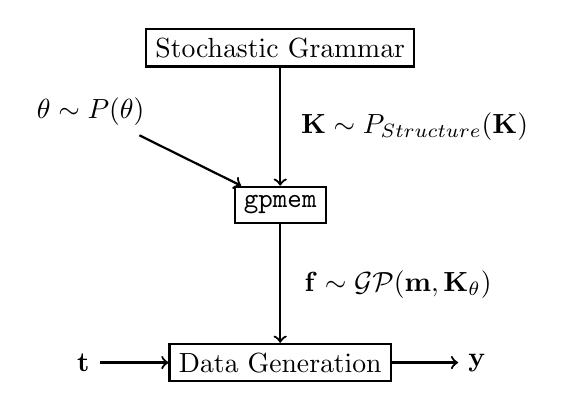
\begin{tikzpicture}[thick]
 \node[draw,rectangle] (grammar) {Stochastic Grammar};
 \node[below left of=grammar,xshift=-1.7cm,yshift=-0.1cm] (theta) {$\bm{\theta} \sim P(\bm{\theta})$};
 \node[draw,rectangle,below of=grammar,yshift=-1cm] (gpmem) {\texttt{gpmem}};
 \node[draw,rectangle,below of=gpmem,yshift=-1cm] (f) {Data Generation};
 \node[below right of=grammar,xshift=1cm,yshift=-0.3cm] (k) {$\mathbf{K} \sim P_{Structure}(\mathbf{K})$};
\node[below right of=gpmem,xshift=0.79cm,yshift=-0.3cm] (gp) {$\mathbf{f} \sim \mathcal{GP}(\mathbf{m},\mathbf{K}_{\bm{\theta}})$};
\node[left of=f,xshift=-1.5cm] (x) {$\mathbf{t}$};
\node[right of=f,xshift=1.5cm] (y) {$\mathbf{y}$};

% 1st pass: draw arrows
  \draw[thick,->] (grammar) -- (gpmem);
  \draw[thick,->] (theta) -- (gpmem);
  \draw[thick,->] (gpmem) -- (f);
 \draw[thick,->] (x) -- (f);
 \draw[thick,->] (f) -- (y);
  % Note: If you have no branches, the 2nd pass is not needed
\end{tikzpicture}
\caption{} 
\end{subfigure}
\begin{subfigure}[b]{0.49\textwidth}\centering
\begin{tikzpicture}[grow=right, sloped]
\node[operator] {\small $+$}
    child {
        node[operator] {\small $\times$}        
            child {
               node[operator] {\small $+$}        
        child {
                node[operator, label=right:
                    {$\cdots$}] {}
                edge from parent
                node[above] {}
                node[below]  {}
            }
            child {
                node[end, label=right:
                    {$\mathbf{K}_4$}] {}
                edge from parent
                node[above] {}
                node[below]  {}
            }
        edge from parent         
            node[above] {}
            node[below]  {}
            }
            child {
                node[end, label=right:
                    {$\mathbf{K}_3$}] {}
                edge from parent
                node[above] {}
                node[below]  {}
            }
            edge from parent 
            node[above] {}
            node[below]  {}
    }
    child {
        node[operator] {\small $+$}        
        child {
                node[end, label=right:
                    {$\mathbf{K}_2$}] {}
                edge from parent
                node[above] {}
                node[below]  {}
            }
            child {
                node[end, label=right:
                    {$\mathbf{K}_1$}] {}
                edge from parent
                node[above] {}
                node[below]  {}
            }
        edge from parent         
            node[above] {}
            node[below]  {}
    };
\node[xshift=-1cm] (K) {$\mathbf{K}=$}; 
 \node[xshift=2.6cm,below =2.4cm of K] (Keq) {$\mathbf{K}=\mathbf{K}_1+\mathbf{K}_2+\mathbf{K}_3 \times (\mathbf{K}_4+\cdots)$};
\end{tikzpicture}
\caption{} 
\end{subfigure}
